%%%%%%%%%%%%%%%%%%%%%%%%%%%%%%%%%%%%%%%%%
% Beamer Presentation
% LaTeX Template
% Version 2.0 (27/IX/15)
%
% This template has been downloaded from http://www.LaTeXTemplates.com
% and modified by Semen Martynov <semen.martynov@gmail.com>
%
% License:
% CC BY-NC-SA 3.0 (http://creativecommons.org/licenses/by-nc-sa/3.0/)
%
%%%%%%%%%%%%%%%%%%%%%%%%%%%%%%%%%%%%%%%%%

%----------------------------------------------------------------------------------------
%	PACKAGES AND THEMES
%----------------------------------------------------------------------------------------

\documentclass{beamer}

\mode<presentation> {

% The Beamer class comes with a number of default slide themes
% which change the colors and layouts of slides. Below this is a list
% of all the themes, uncomment each in turn to see what they look like.

%\usetheme{default}
%\usetheme{AnnArbor}
%\usetheme{Antibes}
%\usetheme{Bergen}
%\usetheme{Berkeley}
%\usetheme{Berlin}
%\usetheme{Boadilla}
%\usetheme{CambridgeUS}
%\usetheme{Copenhagen}
%\usetheme{Darmstadt}
%\usetheme{Dresden}
%\usetheme{Frankfurt}
%\usetheme{Goettingen}
%\usetheme{Hannover}
%\usetheme{Ilmenau}
%\usetheme{JuanLesPins}
%\usetheme{Luebeck}
\usetheme{Madrid}
%\usetheme{Malmoe}
%\usetheme{Marburg}
%\usetheme{Montpellier}
%\usetheme{PaloAlto}
%\usetheme{Pittsburgh}
%\usetheme{Rochester}
%\usetheme{Singapore}
%\usetheme{Szeged}
%\usetheme{Warsaw}

% As well as themes, the Beamer class has a number of color themes
% for any slide theme. Uncomment each of these in turn to see how it
% changes the colors of your current slide theme.

%\usecolortheme{albatross}
%\usecolortheme{beaver}
%\usecolortheme{beetle}
%\usecolortheme{crane}
%\usecolortheme{dolphin}
%\usecolortheme{dove}
%\usecolortheme{fly}
%\usecolortheme{lily}
%\usecolortheme{orchid}
%\usecolortheme{rose}
%\usecolortheme{seagull}
%\usecolortheme{seahorse}
%\usecolortheme{whale}
%\usecolortheme{wolverine}

%\setbeamertemplate{footline} % To remove the footer line in all slides uncomment this line
%\setbeamertemplate{footline}[page number] % To replace the footer line in all slides with a simple slide count uncomment this line

%\setbeamertemplate{navigation symbols}{} % To remove the navigation symbols from the bottom of all slides uncomment this line
\setbeamertemplate{caption}[numbered] % Image numbers
}

%%%% Charset (don't forget about texlive-lang-cyrillic)
\usepackage{cmap}							% make PDF files searchable and copyable
\usepackage[utf8x]{inputenc}				% accept different input encodings
\usepackage[T2A]{fontenc}					% russian font
\usepackage[russian]{babel}					% multilingual support (T2A)

%%%% Graphics
%\usepackage[dvipsnames]{xcolor}			% driver-independent color extensions
\usepackage{graphicx}						% enhanced support for graphics
\usepackage{wrapfig}						% produces figures which text can flow around

%%%% Math
\usepackage{amsmath}						% American Mathematical Society (AMS) math facilities
\usepackage{amsfonts}						% fonts from the AMS
\usepackage{amssymb}						% additional math symbols

%%%% Typograpy (don't forget about cm-super)
\usepackage{microtype}						% subliminal refinements towards typographical perfection
%\linespread{1.3}							% line spacing
\setlength{\parindent}{0pt}					% we don't want any paragraph indentation
\usepackage{parskip}						% some distance between paragraphs

%%%% Tables
\usepackage{booktabs}						% Allows the use of \toprule, \midrule and \bottomrule in tables
%\usepackage{tabularx}						% tables with variable width columns
%\usepackage{multirow}						% for tabularx
%\usepackage{hhline}							% for tabularx

%%%% Graph
%\usepackage{tikz}							% package for creating graphics programmatically
%\usetikzlibrary{arrows}						% edges for tikz

%%%% Other
%\usepackage{url}							% verbatim with URL-sensitive line breaks
%\usepackage{fancyvrb}						% sophisticated verbatim text (with box)

\makeatletter
\def\verbatim{\tiny\@verbatim \frenchspacing\@vobeyspaces \@xverbatim}
\makeatother

%----------------------------------------------------------------------------------------
%	TITLE PAGE
%----------------------------------------------------------------------------------------

\title[Branch Target Buffer]{Исследование характеристик динамического \\ предсказания ветвлений в конвейере с \\ использованием BTB (Branch Target Buffer)} % The short title appears at the bottom of every slide, the full title is only on the title page

\author{Чёрная команда} % Your name
\institute[СПбПУ] % Your institution as it will appear on the bottom of every slide, may be shorthand to save space
{
Санкт-Петербургский политехнический университет Петра Великого \\ % Your institution for the title page
\medskip
\textit{Антон Абрамов <abramov91@mail.ru>\\
Владислав Бусаров <happyfanik@yandex.ru>\\
Сергей Дедков <dsv.mail@yandex.ru>\\
Семён Мартынов <semen.martynov@gmail.com>\\
Николай Патраков <noon.vlg@gmail.com>} % Your email address
}
\date{\today} % Date, can be changed to a custom date

\begin{document}

\begin{frame}
\titlepage % Print the title page as the first slide
\end{frame}

\begin{frame}
\frametitle{Содержание} % Table of contents slide, comment this block out to remove it
\tableofcontents % Throughout your presentation, if you choose to use \section{} and \subsection{} commands, these will automatically be printed on this slide as an overview of your presentation
\end{frame}

%----------------------------------------------------------------------------------------
%	PRESENTATION SLIDES
%----------------------------------------------------------------------------------------

%------------------------------------------------
\section{Принципы конвейеризации}
%------------------------------------------------

\begin{frame}
\frametitle{Принципы конвейеризации}

Существует два подхода к увеличению быстродействия системы:

\begin{itemize}
\item Параллелизм — при параллельной обработке происходит совмещение во времени однотипных операций, выполняемых над разными блоками данных.
\item Конвейеризация — при конвейерной обработке происходит совмещение разнородных вычислительных операций.
\end{itemize}

\begin{block}{Конвейер —}

способ организации вычислений, используемый в современных процессорах и контроллерах с целью повышения их производительности (увеличения числа инструкций, выполняемых в единицу времени), технология, используемая при разработке компьютеров и других цифровых электронных устройств.
\end{block}
 
\end{frame}
%------------------------------------------------

\begin{frame}

Используется конвейерный принцип обработки информации с целью увеличения быстродействия процессора и максимального использования всех его возможностей в современных микропроцессорах. Выполнение каждой команды складывается из ряда последовательных этапов, суть которых не меняется от команды к команде. 

Этот принцип подразумевает, что в каждый момент времени процессор работает над различными стадиями выполнения нескольких команд, причем на выполнение каждой стадии выделяются отдельные аппаратные ресурсы. По очередному тактовому импульсу каждая команда в конвейере продвигается на следующую стадию обработки, выполненная команда покидает конвейер, а новая поступает в него.

\end{frame}
%------------------------------------------------

\begin{frame}
\frametitle{Принципы конвейеризации}

В различных процессорах количество и суть этапов различаются.

Рассмотрим принципы конвейерной обработки информации на примере пятиступенчатого конвейера, в котором выполнение команды складывается из следующих этапов:

IF ( INsTRuction Fetch ) - считывание команды в процессор;

ID ( INsTRuction DecodINg ) - декодирование команды;

OR ( Operand ReadINg ) - считывание операндов;

EX ( ExecutINg ) - выполнение команды;

WB ( Write Back ) - запись результата.

\end{frame}

%------------------------------------------------

\begin{frame}
\frametitle{Принципы конвейеризации}

\begin{figure}
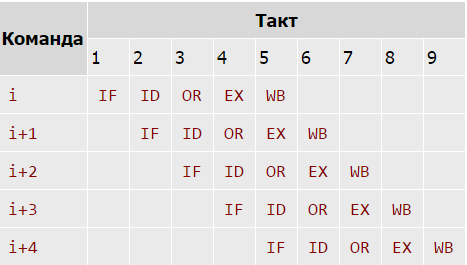
\includegraphics[scale=0.9]{Pic_1}
\caption{Порядок выполнения команд в 5-ступенчатом конвейре}
\end{figure}

\end{frame}
%------------------------------------------------
\section{Конфликты в конвейере}
%------------------------------------------------

\begin{frame}
\frametitle{Конфликты в конвейере}
Значительное преимущество конвейерной обработки перед последовательной имеет место в идеальном конвейере, в котором отсутствуют конфликты и все команды выполняются друг за другом в установившемся режиме, то есть без перезагрузки конвейера. Наличие конфликтов в конвейере и его перезагрузки снижают реальную производительность конвейера по сравнению с идеальным случаем.

\begin{block}{Конфликты —}

это такие ситуации в конвейерной обработке, которые препятствуют выполнению очередной команды в предназначенном для нее такте.
\end{block}
\end{frame}

%------------------------------------------------

\begin{frame}
\frametitle{Конфликты в конвейере}

Конфликты делятся на три группы:

\begin{itemize}
\item структурные;
\item по данным;
\item по управлению.

\end{itemize}

Структурные конфликты вызваны недостаточностью ресурсов вычислительной системы для обеспечения и обработки возможных комбинаций команд.

Конфликт по данным возникает при наличии логических межкомандных зависимостей, т.е. при использовании одной командой результата выполнения другой команды.

\end{frame}

%------------------------------------------------

\begin{frame}
\frametitle{Конфликты по управлению}

Конфликты по управлению связаны с изменением линейной последовательности команд. В конвейерах конфликт возникает из-за вычисления логического условия перехода и задержки получения целевого адреса перехода.

\begin{figure}
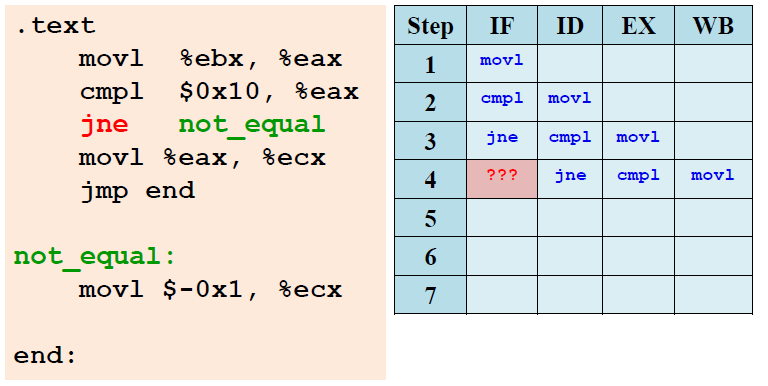
\includegraphics[scale=0.4]{Pic_6}
\end{figure}

В процессоре присутствует модуль предсказания переходов (Branch Prediction Unit).

\end{frame}

%------------------------------------------------
\section{Предсказание переходов}
%------------------------------------------------

\begin{frame}
\frametitle{Предсказание переходов}

Модуль предсказания условных переходов(BranchPredictionUnit, BPU) –модуль процессора,определяющий будет ли выполнен переход и куда.

\begin{itemize}
\item Предсказывает условные переходы, вызовы/возвраты из функций;
\item Вероятность предсказания переходов в современных процессорах превышает 0.9;
\item Альтернативный подход (без BPU) - выполнять обе ветви ветвления, пока не будет вычислено управляющее выражение (условие).
\end{itemize}
Типы предсказания переходов:
\begin{itemize}
\item Статическое предсказание переходов
\item Динамическое предсказание переходов
\end{itemize}
\end{frame}

%------------------------------------------------
\section{Статическое предсказание переходов}
%------------------------------------------------

\begin{frame}
\frametitle{Статическое предсказание переходов}

\begin{block}{Статическое предсказание (Static prediction) –}

фиксированное правило работы предсказателя – условный переход либо выполняются всегда, либо не выполняются никогда.
\end{block}

Статические методы предсказания используются когда невозможно задействовать динамические.

К статическим методам можно отнести:
\begin{itemize}
\item Возврат. Статическое прогнозирование перехода как: всегда выполняемого, либо – всегда не выполняемого.
\item Разворачивание циклов.
\end{itemize}

\end{frame}

%------------------------------------------------
\section{Динамическое предсказание переходов}
%------------------------------------------------

\begin{frame}
\frametitle{Динамические предсказание переходов}

\begin{block}{Динамическое предсказание (Dynamic prediction) –}

осуществляет предсказание направления переходов на основании результатов предыдущих выполнений данной команды.
\end{block}

При использовании этих методов для команд условных переходов анализируется предыстория переходов - результаты нескольких предыдущих команд ветвления по данному адресу. В этом случае возможно определение чаще всего реализуемого направления ветвления, а также выявление чередующихся переходов.

Информация о предыдущих ветвленияххранится в буфере предсказания переходов (Branch Target Buffer – BTB).

\end{frame}

%------------------------------------------------
\section{Branch Target Buffer}
%------------------------------------------------

\begin{frame}
\frametitle{Branch Target Buffer}

\begin{block}{Branch Target Buffer (BTB) –}

это ассоциативный массив (хештаблица) сопоставляющий адресу инструкции ветвления историю переходов и адрес перехода.
\end{block}

На этапе Fetch по адресу инструкции (по IP–Instr. Pointer) происходит обращение в BTB,если запись для IP есть, значит загруженная инструкция –это ветвлениеи в BTB имеется адрес перехода (target address).

\begin{figure}
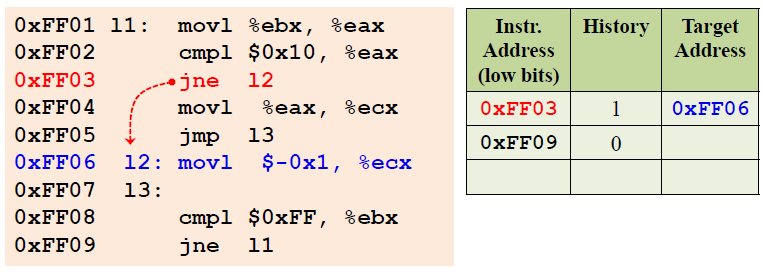
\includegraphics[scale=0.5]{Pic_2}
\caption{Branch Target Buffer}
\end{figure}

\end{frame}

%------------------------------------------------

\begin{frame}

\frametitle{Branch History (1 bit)}


\begin{itemize}
\item 0–ветвление не состоялось, не осуществлять переход;
\item 1–ветвление состоялось, осуществлять переход.
\end{itemize}


\begin{figure}
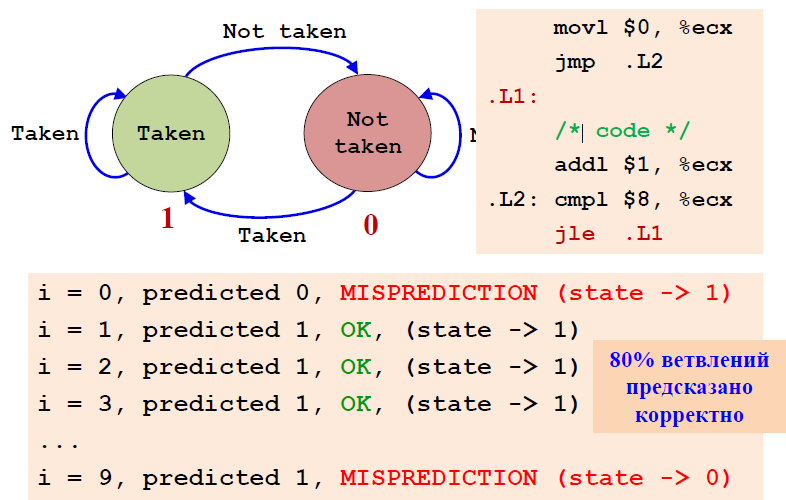
\includegraphics[scale=0.45]{Pic_3}
\end{figure}

\end{frame}


%------------------------------------------------

\begin{frame}
\frametitle{Branch History (1 bit)}

\begin{figure}
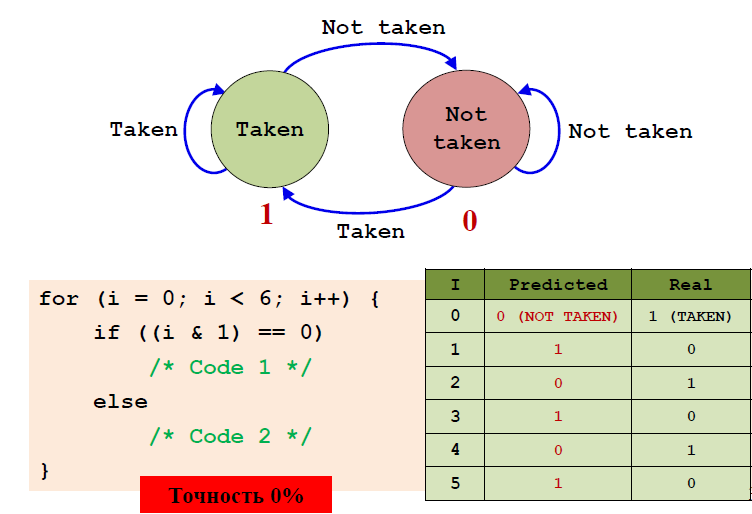
\includegraphics[scale=0.55]{Pic_4}
\end{figure}

\end{frame}

%------------------------------------------------

\begin{frame}

\frametitle{Диаграмма состояний автомата схемы Смита}

Для описания процесса выполнения условных переходов исполь-зуется автомат Мура с 4-мя и более состояниями. Рассмотрим широко применяемый алгоритм Смита с двухразрядными счетчиками. В со-ответствии с ним ведется таблица истории переходов для каждой ус-ловной команды, содержащая по 2 бита на команду.

\begin{figure}
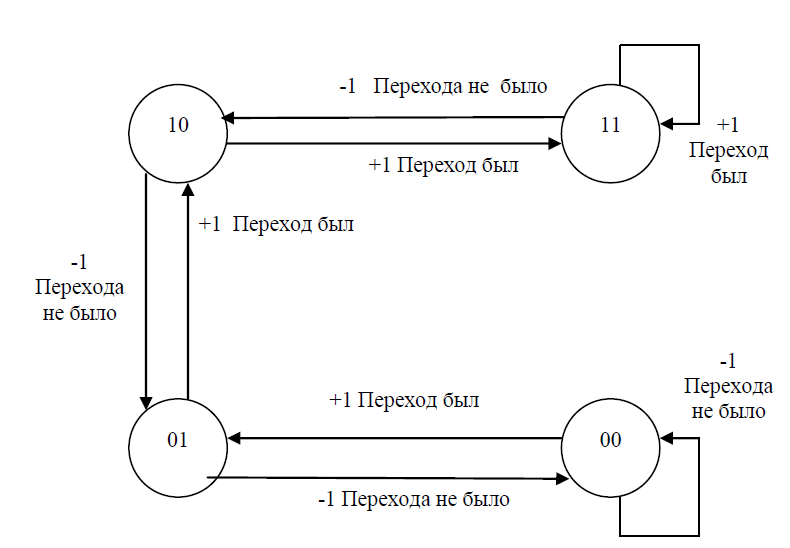
\includegraphics[scale=0.35]{Pic_5}
\end{figure}

\end{frame}

%------------------------------------------------
\section{Эксперимент}
%------------------------------------------------
\begin{frame}
\frametitle{Эксперимент}

Задание 3. 
Исследование характеристик динамического предсказания ветвлений в конвейере с использованием BTB = Branch Target Buffer при разных размерах ВТВ, от 8 до 128 строк. 
На той же вычислительной нагрузке.

\end{frame}

%------------------------------------------------

\begin{frame}
\frametitle{Ливерморские циклы}
"Ливерморские циклы" появился в середине 60-х годов и состоит из фрагментов программ, имеющих реальное хождение в Ливерморской Национальной лаборатории им. Лоуренса в США.\\~\\

Считается, что Ливерморские циклы -- это типичный набор программ для решения численных задач. В этих фрагментах используются различные вычислительные алгоритмы: сеточные, последовательные, волновые, что существенно с точки зрения соответствия вычислительных и аппаратных структур.
\end{frame}

%------------------------------------------------

\begin{frame}
\frametitle{Ливерморские циклы}
\begin{enumerate}
\item Hydro fragment
\item ICCG excerpt (Incomplete Cholesky Conjugate Gradient)
\item Inner product
\item Banded linear equations
\item Tri-diagonal elimination, below diagonal
\item General linear recurrence equations
\item Equation of state fragment
\item ADI integration
\item Integrate predictors
\end{enumerate}
Исходный код \url{https://github.com/SemenMartynov/SPbPU_ComputingSystems/tree/master/lab2/livermorec.txt}
\end{frame}

%------------------------------------------------
\begin{frame}
\frametitle{Результат}

Для изучения характеристик динамического предсказания ветвлений в конвейере, было решено построить модель BPU(Branch Prediction Unit) и использовать информацию о выполнении нагрузки, а именно результат профилирования.

Для получения результатов профилирования был использован pintool: pin-instant. 
https://github.com/wuyongzheng/pin-instat


\end{frame}

%------------------------------------------------
\begin{frame}
\frametitle{Результат}

Профайлер вводит следующую информацию: 

\begin{enumerate}
\item addr - время выполнения
\item opcode	- код команды

\end{enumerate}


\begin{block}{Пример вывода:}

8048294	push ebx

8048295	sub esp

8048298	call 0x8048320

804829d	add ebx

80482a3	mov eax

80482a9	test eax

80482ab	jz 0x80482b3

\end{block}


\end{frame}

%------------------------------------------------
\begin{frame}[fragile]
\frametitle{Результат}

Всего команд: 118735

Команд перехода: 21905

\begin{block}{Результат выполнения}
\begin{verbatim}

/------------------------------------------------------------\
|Размер BTB |    All  |  Hit  |  Miss |  BTB Hit | Percent   |
|-----------|---------|-------|-------|----------|-----------|
|        8  |   21905 | 9324  | 12581 |     8460 |  38,62    |
|       16  |   21905 | 11930 |  9975 |    10866 |  49,6     |
|       32  |   21905 | 12777 |  9128 |    11179 |  51,03    |
|       64  |   21905 | 17643 |  4262 |    16011 |  73,09    |
|      128  |   21905 | 19274 |  2631 |    17422 |  79,54    |
\------------------------------------------------------------/

\end{verbatim}
\end{block}
\end{frame}

%------------------------------------------------

\begin{frame}
\frametitle{Результат}

\begin{figure}
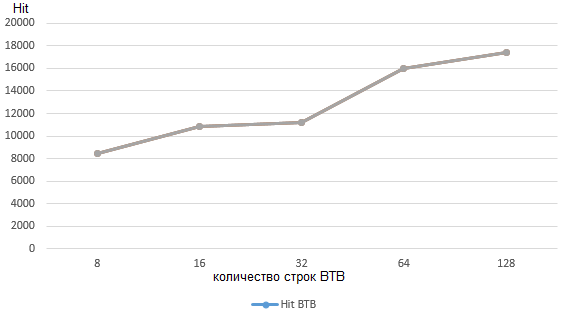
\includegraphics[scale=0.8]{Pic_8}
\end{figure}

\end{frame}

%------------------------------------------------
\begin{frame}
\frametitle{Результат}

\begin{figure}
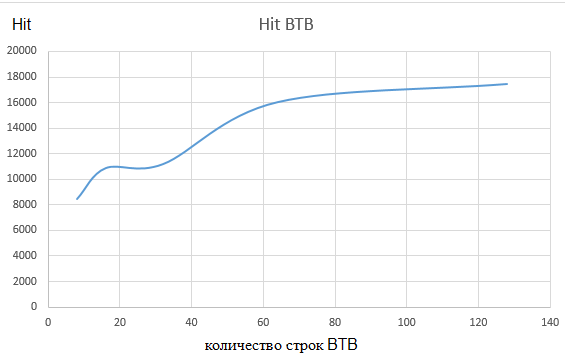
\includegraphics[scale=0.8]{Pic_7}
\end{figure}


\end{frame}

%------------------------------------------------

\begin{frame}
\frametitle{Выводы}

\begin{itemize}
\item Количество команд перехода составляет около 20\%, что означает большую значимость использования BTB.
\item Как видно из результатов эксперимента используя BTB размером менее 32 строк не имеет смысла, а BTB больше 64 строк уеличивает процент попадания с ростом строк BTB незначительно. Следовательно, оптимальный размер BTB для данного эксперимента от 32 до 64 строк.
\end{itemize}

\end{frame}


%------------------------------------------------
\section{Вопросы}
%------------------------------------------------

\begin{frame}
\Huge{\centerline{Вопросы?}}
\end{frame}

%----------------------------------------------------------------------------------------

\end{document}